\documentclass[conference]{IEEEtran}

% === Packages ===
\usepackage[utf8]{inputenc}
\usepackage[T1]{fontenc}
\usepackage{amsmath,amssymb}
\usepackage{graphicx}
\usepackage{booktabs}
\usepackage{multirow}
\usepackage{array}
\usepackage{url}
\usepackage{hyperref}
\usepackage{xcolor}
\usepackage[caption=false]{subfig}
\usepackage{tikz}
\usetikzlibrary{shapes.geometric, arrows.meta, positioning, fit, calc, backgrounds, decorations.pathreplacing}

% === TikZ styles ===
\tikzset{
  % Flowchart styles
  startstop/.style={rectangle, rounded corners=6pt, minimum width=2.4cm, minimum height=0.7cm, text centered, draw=black, fill=green!15, font=\scriptsize},
  process/.style={rectangle, minimum width=2.8cm, minimum height=0.7cm, text centered, draw=black, fill=blue!8, font=\scriptsize},
  decision/.style={diamond, aspect=2.2, minimum width=1.2cm, minimum height=0.6cm, text centered, draw=black, fill=orange!15, font=\scriptsize},
  io/.style={trapezium, trapezium left angle=70, trapezium right angle=110, minimum width=2cm, minimum height=0.6cm, text centered, draw=black, fill=yellow!12, font=\scriptsize},
  arrow/.style={-{Stealth[length=2mm]}, thick},
  % Architecture diagram styles
  block/.style={rectangle, rounded corners=3pt, minimum width=1.6cm, minimum height=0.6cm, text centered, draw=black, fill=#1, font=\scriptsize},
  block/.default={blue!12},
  smallblock/.style={rectangle, rounded corners=2pt, minimum width=1.2cm, minimum height=0.5cm, text centered, draw=black, fill=#1, font=\tiny},
  smallblock/.default={blue!12},
  bigblock/.style={rectangle, rounded corners=4pt, minimum width=2.2cm, minimum height=0.7cm, text centered, draw=black, fill=#1, font=\scriptsize},
  bigblock/.default={blue!12},
  group/.style={rectangle, rounded corners=4pt, draw=gray, dashed, inner sep=6pt},
}

% === Figure placeholder command (for images only) ===
\newcommand{\figplaceholder}[2]{%
  \begin{center}
    \fbox{\parbox{0.9\linewidth}{\centering\vspace{1.2cm}\textbf{#1}\\[3pt]\small #2\vspace{1.2cm}}}
  \end{center}
}

\begin{document}

% === Title ===
\title{CropPlanner: An AI-Powered Web Application for Crop Planning Recommendations}

\author{
  \IEEEauthorblockN{Thatt Bunnag\IEEEauthorrefmark{1}, Nathanon Ratchathornbuathip\IEEEauthorrefmark{1}, Art-ong Mukngoen\IEEEauthorrefmark{2}, Atthaphon Lorphan\IEEEauthorrefmark{2}}
  \IEEEauthorblockA{Chitralada School, Bangkok, Thailand \\
  \IEEEauthorrefmark{1}Students \quad \IEEEauthorrefmark{2}Advisors}
}

\maketitle

% ============================================================
% ABSTRACT
% ============================================================
\begin{abstract}
Agricultural price volatility exceeding 20\% annually, combined with the prevalence of monoculture farming practices, exposes Thai farmers to significant income risks. This paper presents CropPlanner, an integrated system comprising three components: (1)~a comparative study of AI models for 12-month crop price forecasting, including LSTM, Transformer, ARIMA, and a proposed Rolling-Window LSTM; (2)~a crop planning recommendation system formulated as a Weighted Job Scheduling Problem solved by a Greedy Heuristic; and (3)~a web application for farmers. Experiments were conducted using 20~years of monthly price data (2004--2024) for four major field crops---cassava, corn, green bean, and soybean---in Northeastern Thailand. Results show that no single model dominates across all crops: Standard LSTM achieved the highest average accuracy of 92.93\%, while Rolling-Window LSTM excelled in peak timing accuracy, predicting peak price months within one month for three out of four crops---a property critical for scheduling. The Greedy Scheduling system produced a non-overlapping four-crop rotation plan yielding 41,377~THB/rai/year, approximately 2.4~times the income of the best monoculture option.
\end{abstract}

\begin{IEEEkeywords}
Machine Learning, Price Forecasting, Web Application, Time Series, ARIMA, LSTM, Transformer, Crop Planning
\end{IEEEkeywords}

% ============================================================
% I. INTRODUCTION
% ============================================================
\section{Introduction}

Agriculture forms a critical foundation of the Thai economy. Four major field crops---cassava, corn, green bean, and soybean---account for over 60\% of cultivated land and generate export revenues exceeding US\$13~billion annually~\cite{oae2024stats, oae2024forecast, ocsb2024, thairice2024}. However, prices of these crops exhibit volatility exceeding 20\% within a 12-month period~\cite{waqas2024climate}, creating substantial income risks for farmers.

A key contributing factor is the widespread practice of monoculture farming. Many farmers plant the same crop continuously throughout the year, leaving them vulnerable when prices decline during certain periods~\cite{asg2014}. While government price support programs provide temporary relief, they are insufficient for long-term income stabilization. What farmers fundamentally lack are tools for forward-looking price forecasting and systematic planting schedule optimization.

Recent advances in Machine Learning, particularly time-series models such as LSTM and Transformer, have demonstrated the ability to reduce Mean Absolute Error (MAE) in agricultural price prediction by up to 35\% compared to traditional methods~\cite{rohan2025crop}. Yet most existing work focuses on forecasting individual crop prices in isolation, without connecting predictions to actionable planting recommendations~\cite{javaid2023ai}.

This paper presents CropPlanner, an end-to-end system linking AI-based price forecasting with crop scheduling and a farmer-facing web application. Our contributions are threefold:

\begin{enumerate}
  \item \textbf{Model comparison and improvement:} We compare LSTM, Transformer, ARIMA, and a proposed Rolling-Window LSTM for 12-month price forecasting of four Thai field crops, analyzing both overall accuracy and peak timing accuracy.
  \item \textbf{Crop planning recommendation:} We formulate planting schedule optimization as a Weighted Job Scheduling Problem and solve it with a Greedy Heuristic that produces non-overlapping planting--harvest timelines.
  \item \textbf{Web application:} We develop CropPlanner, a prototype web application that presents forecasting results and planting recommendations through intuitive visualizations.
\end{enumerate}

% --- Fig. 1: System Overview ---
\begin{figure}[htbp]
  \centering
  \resizebox{\columnwidth}{!}{%
  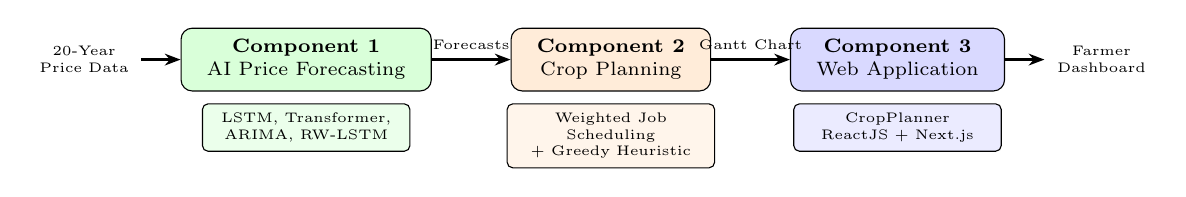
\begin{tikzpicture}[node distance=0.4cm]
    % Component 1
    \node[bigblock=green!15] (ai) {
      \begin{tabular}{c}
        \textbf{Component 1}\\
        AI Price Forecasting
      \end{tabular}
    };
    \node[smallblock=green!8, below=0.15cm of ai, text width=2.4cm, align=center] (aidet) {LSTM, Transformer,\\ARIMA, RW-LSTM};

    % Component 2
    \node[bigblock=orange!15, right=1.0cm of ai] (sched) {
      \begin{tabular}{c}
        \textbf{Component 2}\\
        Crop Planning
      \end{tabular}
    };
    \node[smallblock=orange!8, below=0.15cm of sched, text width=2.4cm, align=center] (scheddet) {Weighted Job Scheduling\\+ Greedy Heuristic};

    % Component 3
    \node[bigblock=blue!15, right=1.0cm of sched] (web) {
      \begin{tabular}{c}
        \textbf{Component 3}\\
        Web Application
      \end{tabular}
    };
    \node[smallblock=blue!8, below=0.15cm of web, text width=2.4cm, align=center] (webdet) {CropPlanner\\ReactJS + Next.js};

    % Arrows
    \draw[arrow] (ai) -- node[above, font=\tiny] {Forecasts} (sched);
    \draw[arrow] (sched) -- node[above, font=\tiny] {Gantt Chart} (web);

    % Input/Output
    \node[left=0.5cm of ai, font=\tiny, text width=1.2cm, align=center] (input) {20-Year\\Price Data};
    \node[right=0.5cm of web, font=\tiny, text width=1.2cm, align=center] (output) {Farmer\\Dashboard};
    \draw[arrow] (input) -- (ai);
    \draw[arrow] (web) -- (output);
  \end{tikzpicture}}
  \caption{System overview of CropPlanner comprising three integrated components.}
  \label{fig:system}
\end{figure}

% ============================================================
% II. RELATED WORK
% ============================================================
\section{Related Work}

\subsection{Time-Series Forecasting for Agricultural Prices}

Agricultural price forecasting has been extensively studied using statistical and machine learning approaches. Traditional ARIMA models remain widely used for linear time-series data but struggle with structural breaks and nonlinear patterns. Deep learning models have gained prominence, with LSTM networks---designed to capture long-term dependencies through gating mechanisms~\cite{hochreiter1997lstm}---and Transformer architectures---leveraging self-attention to process entire sequences simultaneously~\cite{vaswani2017attention}---showing superior performance on various forecasting benchmarks.

Rohan~\cite{rohan2025crop} demonstrated that LSTM and Transformer models can reduce MAE by up to 35\% compared to traditional methods for crop price prediction. Javaid et al.~\cite{javaid2023ai} surveyed AI applications in agriculture broadly, including predictive analytics. However, most prior work forecasts a single crop in isolation and does not connect predictions to downstream planning systems.

\subsection{Crop Scheduling and Decision Support Systems}

Resource allocation in agriculture can be modeled as optimization problems such as the Knapsack Problem for area allocation or Job Scheduling for temporal planning. Agricultural Decision Support Systems (DSS) have been developed in various contexts but typically rely on static agronomic data---planting calendars or soil information---rather than AI-driven price forecasts as decision variables.

The gap that this work addresses is the integration of AI price forecasting with scheduling optimization and farmer-accessible web delivery---a pipeline that, to our knowledge, has not been presented as a unified system in prior literature.

% ============================================================
% III. DATA AND PREPROCESSING
% ============================================================
\section{Data and Preprocessing}

\subsection{Data Sources}

Price data were obtained from two Thai government agencies: the Department of Internal Trade (DIT) and the Office of Agricultural Economics (OAE). Table~\ref{tab:dataset} summarizes the dataset.

\begin{table}[htbp]
  \centering
  \caption{Dataset Summary}
  \label{tab:dataset}
  \begin{tabular}{ll}
    \toprule
    \textbf{Property} & \textbf{Value} \\
    \midrule
    Crops & Cassava, Corn, Green Bean, Soybean \\
    Region & Northeastern Thailand \\
    Period & Jan 2004 -- Dec 2024 (20 years) \\
    Frequency & Monthly \\
    Records & $\sim$252 per crop \\
    Currency & Thai Baht (THB/kg) \\
    \bottomrule
  \end{tabular}
\end{table}

\subsection{Preprocessing}

Raw data in PDF and Excel format with Thai Buddhist Era dates underwent several cleaning steps: date conversion from Buddhist Era (BE) to Common Era (CE), duplicate removal, and unit normalization. Processing was performed using Python with Pandas and NumPy. The final cleaned data was stored in long-format CSV files with \texttt{date} and \texttt{price} columns.

\figplaceholder{Fig.~2: Historical Price Trends}{20-year price trends (2004--2024) for four crops showing seasonal patterns and structural breaks. \textit{(Replace with actual plot from repository)}}

\subsection{Train--Test Split}

Data was split into a training set (2004--2023) and a test set (2024 only). The scaler was fit exclusively on training data to prevent data leakage. No separate validation set was used; hyperparameters were fixed \textit{a priori} and not tuned on test results.

% ============================================================
% IV. METHODOLOGY
% ============================================================
\section{Methodology}

The CropPlanner system comprises three components: (A)~AI~price forecasting models, (B)~crop planning recommendation, and (C)~a~web application. All models take 12~months of historical prices as input and produce 12-month forecasts.

\subsection{AI Price Forecasting Models}

Table~\ref{tab:hyperparams} summarizes the hyperparameters of all four models.

\begin{table}[htbp]
  \centering
  \caption{Hyperparameter Summary}
  \label{tab:hyperparams}
  \begin{tabular}{lcccc}
    \toprule
    \textbf{Parameter} & \textbf{LSTM} & \textbf{Trans.} & \textbf{ARIMA} & \textbf{RW-LSTM} \\
    \midrule
    Architecture & 2-layer & 2-layer enc. & Auto & 3-layer \\
    Hidden / $d_{\text{model}}$ & 32 & 64 & auto & 32 \\
    Attn.\ heads & -- & 8 & -- & -- \\
    FF dim & -- & 128 & -- & -- \\
    Epochs & 300 & 500 & -- & 300 \\
    Learning rate & 0.01 & 0.001 & -- & 0.01 \\
    Loss function & MSE & MSE & -- & MSE \\
    Library & PyTorch & PyTorch & StatsFC & PyTorch \\
    \bottomrule
  \end{tabular}
\end{table}

\subsubsection{Standard LSTM}

Long Short-Term Memory (LSTM)~\cite{hochreiter1997lstm} is a recurrent neural network designed to learn long-term dependencies via gating mechanisms (forget, input, and output gates). Our model consists of 2~layers with hidden size~32, receiving 12~months of input and producing 12~months of output. Training used MSE loss on PyTorch for 300~epochs with learning rate~0.01 and random seed~42.

% --- Fig. 3: LSTM Architecture (from code: lstm_model.py) ---
\begin{figure}[htbp]
  \centering
  \resizebox{\columnwidth}{!}{%
  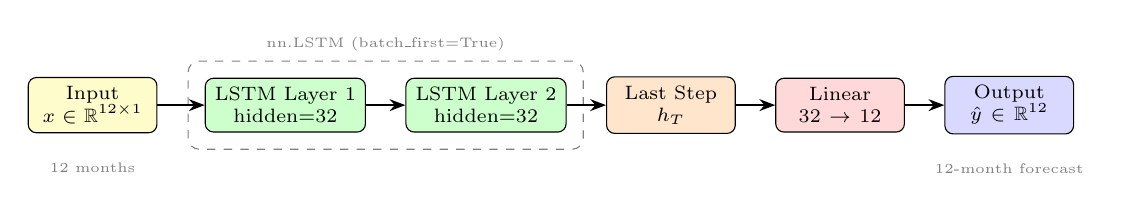
\begin{tikzpicture}[node distance=0.35cm and 0.3cm]
    % Input
    \node[block=yellow!20, text width=1.4cm, align=center] (input) {Input\\$x \in \mathbb{R}^{12 \times 1}$};

    % LSTM layers
    \node[block=green!20, right=0.6cm of input, text width=1.8cm, align=center] (lstm1) {LSTM Layer 1\\hidden=32};
    \node[block=green!20, right=0.5cm of lstm1, text width=1.8cm, align=center] (lstm2) {LSTM Layer 2\\hidden=32};

    % Last hidden state
    \node[block=orange!20, right=0.5cm of lstm2, text width=1.4cm, align=center] (last) {Last Step\\$h_{T}$};

    % FC
    \node[block=red!15, right=0.5cm of last, text width=1.4cm, align=center] (fc) {Linear\\$32 \to 12$};

    % Output
    \node[block=blue!15, right=0.5cm of fc, text width=1.4cm, align=center] (output) {Output\\$\hat{y} \in \mathbb{R}^{12}$};

    % Arrows
    \draw[arrow] (input) -- (lstm1);
    \draw[arrow] (lstm1) -- (lstm2);
    \draw[arrow] (lstm2) -- (last);
    \draw[arrow] (last) -- (fc);
    \draw[arrow] (fc) -- (output);

    % Annotations
    \node[below=0.25cm of input, font=\tiny, text=gray] {12 months};
    \node[below=0.25cm of output, font=\tiny, text=gray] {12-month forecast};

    % Group LSTM
    \begin{scope}[on background layer]
      \node[group, fit=(lstm1)(lstm2), label={[font=\tiny, text=gray]above:nn.LSTM (batch\_first=True)}] {};
    \end{scope}
  \end{tikzpicture}}
  \caption{Standard LSTM architecture. Input sequence of 12 monthly prices passes through 2~LSTM layers (hidden=32). The last time step's hidden state is projected to 12 output values via a linear layer.}
  \label{fig:lstm}
\end{figure}

\subsubsection{Transformer}

The Transformer model~\cite{vaswani2017attention} uses multi-head self-attention to process the entire sequence simultaneously, efficiently capturing global dependencies across time steps. Our encoder-only configuration uses $d_{\text{model}} = 64$, 8~attention heads, 2~layers, and feed-forward dimension~128 with positional encoding. Training ran for 500~epochs at a learning rate of 0.001.

% --- Fig. 4: Transformer Architecture (from code: transformer_model.py) ---
\begin{figure}[htbp]
  \centering
  \resizebox{\columnwidth}{!}{%
  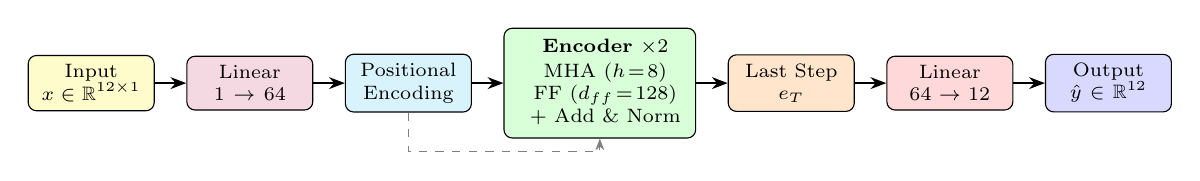
\begin{tikzpicture}[node distance=0.35cm and 0.4cm]
    % Input
    \node[block=yellow!20, text width=1.3cm, align=center] (input) {Input\\$x \in \mathbb{R}^{12 \times 1}$};

    % Input projection
    \node[block=purple!15, right=0.4cm of input, text width=1.3cm, align=center] (proj) {Linear\\$1 \to 64$};

    % Positional Encoding
    \node[block=cyan!15, right=0.4cm of proj, text width=1.3cm, align=center] (pe) {Positional\\Encoding};

    % Encoder block (repeated)
    \node[block=green!15, right=0.4cm of pe, text width=2.2cm, align=center, minimum height=1.2cm] (enc) {
      \begin{tabular}{c}
        \textbf{Encoder} $\times 2$\\[1pt]
        MHA ($h\!=\!8$)\\
        FF ($d_{ff}\!=\!128$)\\
        + Add \& Norm
      \end{tabular}
    };

    % Last step
    \node[block=orange!20, right=0.4cm of enc, text width=1.2cm, align=center] (last) {Last Step\\$e_{T}$};

    % Decoder
    \node[block=red!15, right=0.4cm of last, text width=1.2cm, align=center] (dec) {Linear\\$64 \to 12$};

    % Output
    \node[block=blue!15, right=0.4cm of dec, text width=1.3cm, align=center] (output) {Output\\$\hat{y} \in \mathbb{R}^{12}$};

    % Arrows
    \draw[arrow] (input) -- (proj);
    \draw[arrow] (proj) -- (pe);
    \draw[arrow] (pe) -- (enc);
    \draw[arrow] (enc) -- (last);
    \draw[arrow] (last) -- (dec);
    \draw[arrow] (dec) -- (output);

    % Add + residual annotation
    \draw[-{Stealth[length=1.5mm]}, gray, dashed] (pe.south) -- ++(0,-0.5) -| (enc.south);
  \end{tikzpicture}}%
  \caption{Transformer architecture (encoder-only). Prices are projected to $d_{\text{model}}=64$, augmented with positional encoding, and processed by 2~encoder layers with 8-head attention. The last position's encoding is decoded to 12~output values.}
  \label{fig:transformer}
\end{figure}

\subsubsection{ARIMA}

ARIMA (Autoregressive Integrated Moving Average)~\cite{boxjenkins} combines autoregressive, differencing, and moving average components. We used AutoARIMA from the StatsForecast library, which automatically selects $(p, d, q)$ parameters through time-series decomposition into trend, seasonality, and residual components.

% --- Fig. 5: ARIMA Pipeline ---
\begin{figure}[htbp]
  \centering
  \resizebox{\columnwidth}{!}{%
  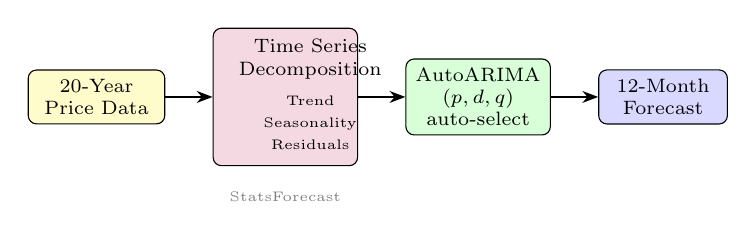
\begin{tikzpicture}[node distance=0.4cm]
    % Data
    \node[block=yellow!20, text width=1.5cm, align=center] (data) {20-Year\\Price Data};

    % Decomposition
    \node[block=purple!15, right=0.6cm of data, text width=1.6cm, align=center, minimum height=1.5cm] (decomp) {
      \begin{tabular}{c}
        Time Series\\Decomposition\\[3pt]
        {\tiny Trend}\\
        {\tiny Seasonality}\\
        {\tiny Residuals}
      \end{tabular}
    };

    % AutoARIMA
    \node[block=green!15, right=0.6cm of decomp, text width=1.6cm, align=center] (arima) {AutoARIMA\\$(p,d,q)$\\auto-select};

    % Output
    \node[block=blue!15, right=0.6cm of arima, text width=1.4cm, align=center] (out) {12-Month\\Forecast};

    % Arrows
    \draw[arrow] (data) -- (decomp);
    \draw[arrow] (decomp) -- (arima);
    \draw[arrow] (arima) -- (out);

    \node[below=0.2cm of decomp, font=\tiny, text=gray] {StatsForecast};
  \end{tikzpicture}}
  \caption{ARIMA forecasting pipeline. Historical data is decomposed into trend, seasonality, and residual components before AutoARIMA selects optimal $(p,d,q)$ parameters.}
  \label{fig:arima}
\end{figure}

\subsubsection{Rolling-Window LSTM (Proposed Improvement)}

Analysis of the standard LSTM revealed three issues: (1)~off-peak prediction---the model misidentified peak price months; (2)~limited long-term dependency over the full 20-year sequence; and (3)~sensitivity to noisy data.

% --- Fig. 6: Rolling-Window Concept ---
\begin{figure}[htbp]
  \centering
  \resizebox{\columnwidth}{!}{%
  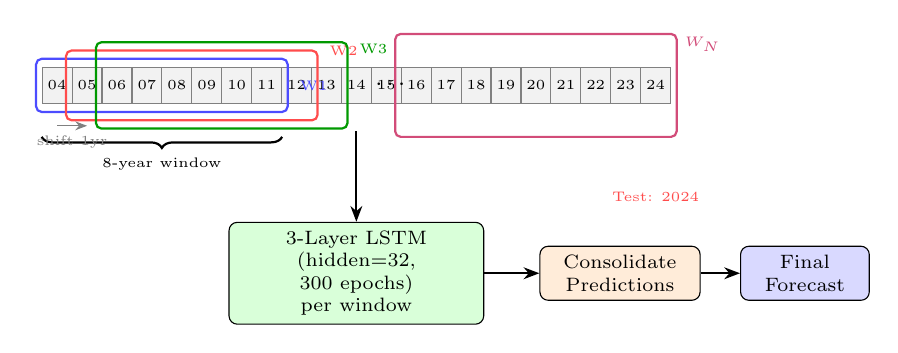
\begin{tikzpicture}[
    yearbox/.style={rectangle, minimum width=0.38cm, minimum height=0.45cm, draw=black!50, font=\tiny, inner sep=1pt},
    winbrace/.style={decorate, decoration={brace, amplitude=4pt, mirror}, thick}
  ]
    % Year boxes
    \foreach \i/\yr in {0/04,1/05,2/06,3/07,4/08,5/09,6/10,7/11,8/12,9/13,10/14,11/15,12/16,13/17,14/18,15/19,16/20,17/21,18/22,19/23,20/24} {
      \node[yearbox, fill=gray!10] (y\i) at (\i*0.38, 0) {\yr};
    }

    % Window 1 (8-year example)
    \draw[thick, blue!70, rounded corners=2pt] ([xshift=-2pt, yshift=3pt]y0.north west) rectangle ([xshift=2pt, yshift=-3pt]y7.south east);
    \node[right=0.1cm of y7, font=\tiny, blue!70] {W1};

    % Window 2
    \draw[thick, red!70, rounded corners=2pt] ([xshift=-2pt, yshift=6pt]y1.north west) rectangle ([xshift=2pt, yshift=-6pt]y8.south east);
    \node[above right=0.02cm and 0.1cm of y8, font=\tiny, red!70] {W2};

    % Window 3
    \draw[thick, green!60!black, rounded corners=2pt] ([xshift=-2pt, yshift=9pt]y2.north west) rectangle ([xshift=2pt, yshift=-9pt]y9.south east);
    \node[above right=0.05cm and 0.1cm of y9, font=\tiny, green!60!black] {W3};

    % Dots
    \node[right=0.3cm of y9, font=\small] (dots) {$\cdots$};

    % Last window
    \draw[thick, purple!70, rounded corners=2pt] ([xshift=-2pt, yshift=12pt]y12.north west) rectangle ([xshift=2pt, yshift=-12pt]y20.south east);
    \node[above right=0.08cm and 0.05cm of y20, font=\tiny, purple!70] {$W_N$};

    % Shift annotation
    \draw[winbrace] ([yshift=-12pt]y0.south west) -- node[below=4pt, font=\tiny] {8-year window} ([yshift=-12pt]y7.south east);

    % Arrow showing shift
    \draw[-{Stealth[length=1.5mm]}, gray] ([yshift=-8pt]y0.south) -- node[below, font=\tiny] {shift 1yr} ([yshift=-8pt]y1.south);

    % Target year
    \node[below=1.0cm of y20, font=\tiny, text=red!70] {Test: 2024};

    % LSTM box below
    \node[block=green!15, below=1.5cm of y10, text width=3cm, align=center] (lstm3) {3-Layer LSTM\\(hidden=32, 300 epochs)\\per window};

    % Consolidate
    \node[block=orange!15, right=0.7cm of lstm3, text width=1.8cm, align=center] (consol) {Consolidate\\Predictions};

    \node[block=blue!15, right=0.5cm of consol, text width=1.4cm, align=center] (final) {Final\\Forecast};

    \draw[arrow] ([yshift=-10pt]y10.south) -- (lstm3);
    \draw[arrow] (lstm3) -- (consol);
    \draw[arrow] (consol) -- (final);
  \end{tikzpicture}}%
  \caption{Rolling-Window LSTM training concept. The 20-year dataset is divided into overlapping windows of 7--8~years, each shifted by 1~year. A 3-layer LSTM is trained on each window independently; predictions are consolidated into a final forecast.}
  \label{fig:rolling}
\end{figure}

To address these issues, we propose the Rolling-Window LSTM. The 20-year dataset is divided into rolling windows of 7--8~years (crop-dependent), each shifted by 1~year. A~3-layer LSTM (hidden size~32, 300~epochs) is trained on each window independently. Predictions from all windows are then consolidated into a final forecast for the target year.

Window sizes were selected through per-crop experimentation: cassava uses a 7-year window, while corn, green bean, and soybean use 8-year windows. By learning from multiple shorter windows, the model captures recurring seasonal patterns more accurately---particularly the location of peak prices, which is critical for the downstream scheduling system.

\figplaceholder{Fig.~7: Standard LSTM vs.\ RW-LSTM Peak Comparison (Green Bean)}{Standard LSTM predicts peak 3~months off; RW-LSTM predicts peak within 1~month. \textit{(Replace with actual comparison plot)}}

\subsubsection{Evaluation Metrics}

Model performance was evaluated using three metrics.

\textit{Mean Absolute Error (MAE):}
\begin{equation}
  \text{MAE} = \frac{1}{n}\sum_{t=1}^{n}|\hat{y}_t - y_t|
\end{equation}

\textit{Mean Absolute Percentage Error (MAPE):}
\begin{equation}
  \text{MAPE} = \frac{100\%}{n}\sum_{t=1}^{n}\left|\frac{\hat{y}_t - y_t}{y_t}\right|
\end{equation}

\textit{Accuracy:}
\begin{equation}
  \text{Accuracy} = 1 - \text{MAPE}
\end{equation}

Additionally, \textbf{Peak Timing Accuracy} was measured for the Rolling-Window LSTM, defined as the absolute difference in months between the predicted and actual peak price positions. This metric is critical because the scheduling system uses peak positions to determine harvest dates.

\subsection{Crop Planning Recommendation System}

The crop planning problem is formulated as a \textit{Weighted Job Scheduling Problem}. Each crop constitutes a job with a duration equal to its growing period and a weight equal to its expected income. The constraint is that no two jobs may overlap on a single plot of land (1~rai = 1,600~m$^2$).

\subsubsection{Phase 1: Job Definition from Forecasts}

Rolling-Window LSTM forecasts are normalized by dividing each crop's price series by its mean, enabling cross-crop comparison. The peak normalized price date~(argmax) defines the harvest date---the optimal selling time. The planting date is then computed by subtracting the growing period:
\begin{equation}
  t_{\text{plant}} = t_{\text{harvest}} - d_{\text{grow}}
\end{equation}

Table~\ref{tab:agro} lists the agronomic constants used.

\begin{table}[htbp]
  \centering
  \caption{Agronomic Constants per Crop}
  \label{tab:agro}
  \begin{tabular}{lcc}
    \toprule
    \textbf{Crop} & \textbf{Growing Days} & \textbf{Yield (kg/rai)} \\
    \midrule
    Cassava & 250 & 3,500 \\
    Corn & 120 & 1,500 \\
    Green Bean & 80 & 245 \\
    Soybean & 90 & 300 \\
    \bottomrule
  \end{tabular}
\end{table}

Each crop's expected income is computed as:
\begin{equation}
  I_i = Y_i \times P_i^{\text{peak}} \times A
\end{equation}
where $Y_i$ is yield (kg/rai), $P_i^{\text{peak}}$ is the price at peak (THB/kg), and $A$ is area (1~rai).

\subsubsection{Phase 2: Greedy Scheduling}

Since independently optimal positions for each crop may overlap, a scheduling algorithm is required. Fig.~\ref{fig:flowchart} presents the greedy scheduling process as a flowchart.

% --- Fig. 8: Greedy Scheduling Flowchart ---
\begin{figure*}[htbp]
  \centering
  \resizebox{\textwidth}{!}{%
  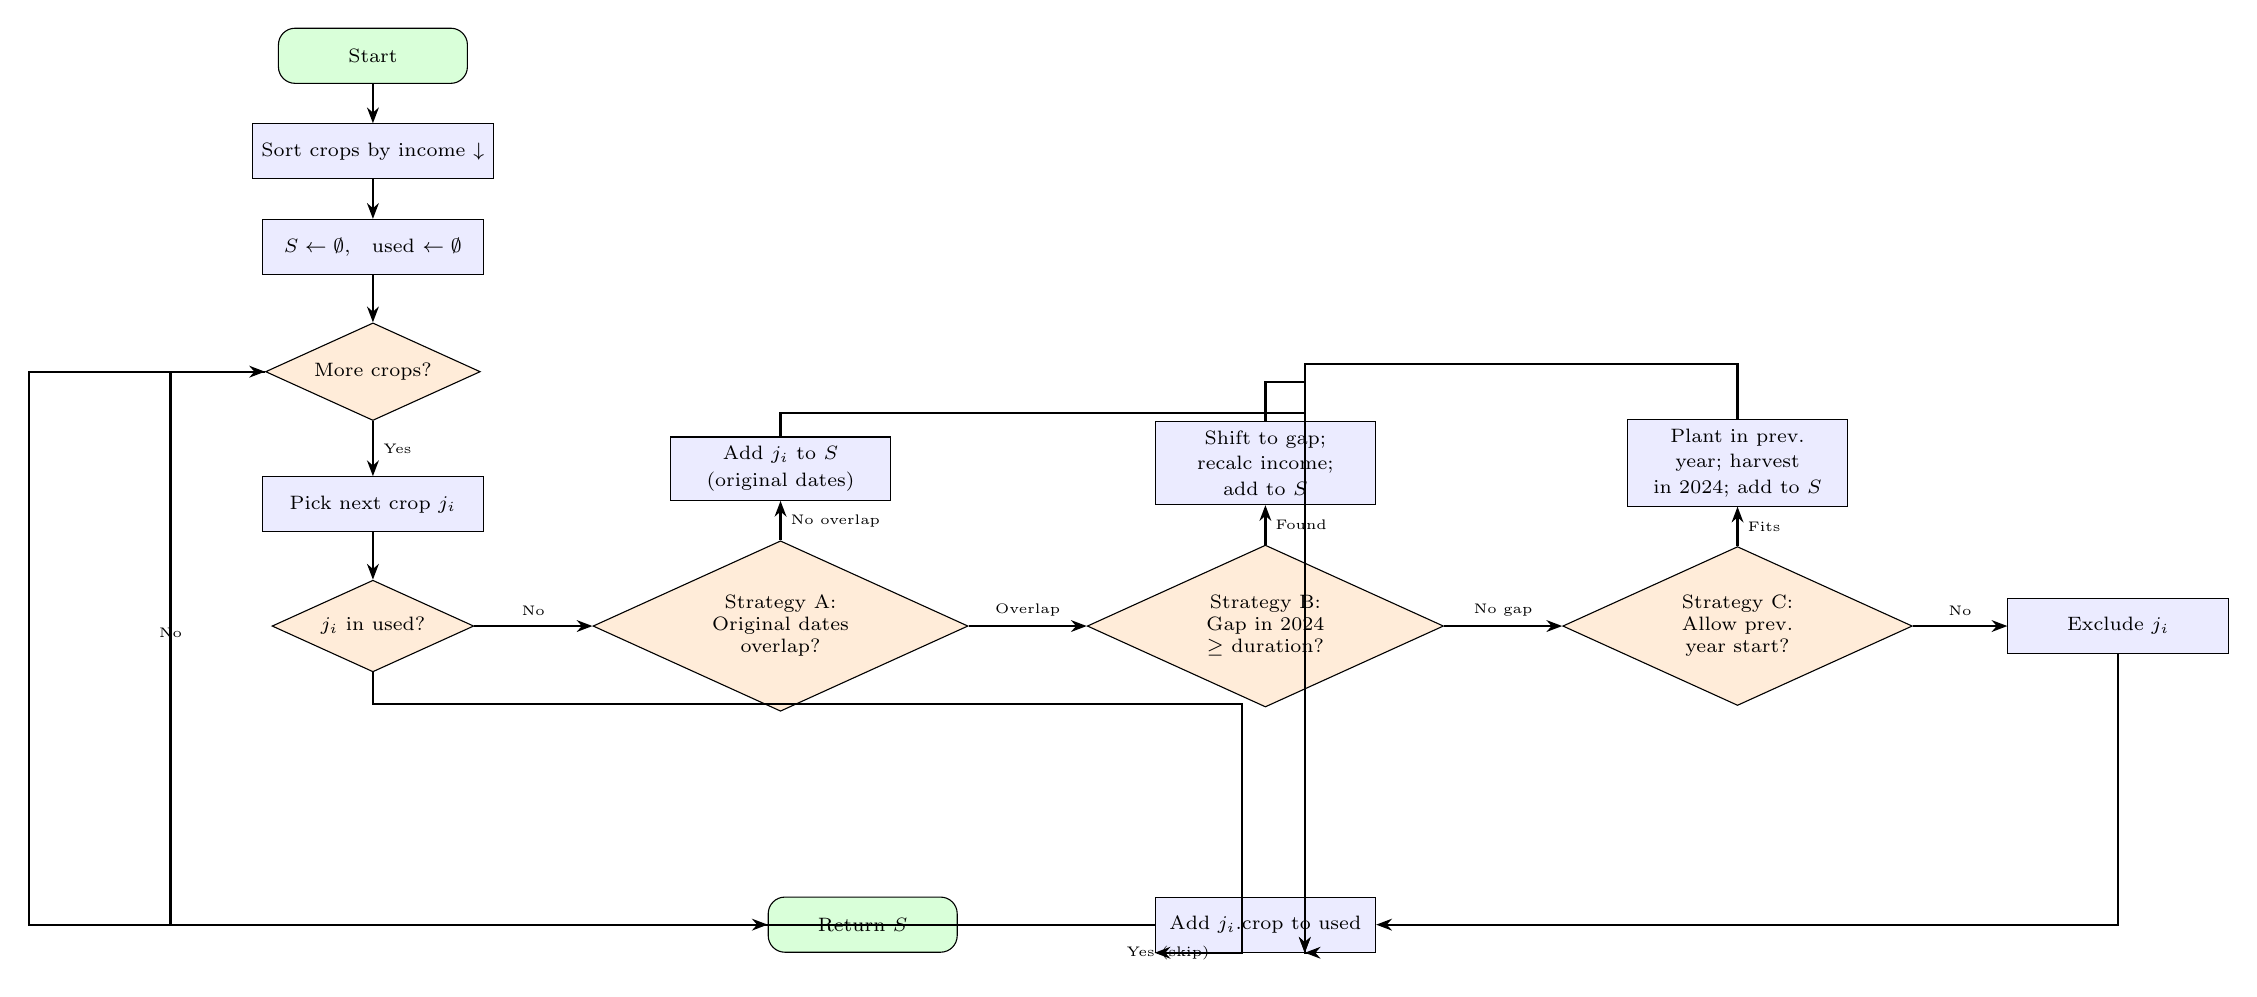
\begin{tikzpicture}[node distance=0.5cm and 0.6cm]
    % Start
    \node[startstop] (start) {Start};

    % Sort
    \node[process, below=0.5cm of start] (sort) {Sort crops by income $\downarrow$};

    % Init
    \node[process, below=of sort] (init) {$S \leftarrow \emptyset$, \; used $\leftarrow \emptyset$};

    % Loop
    \node[decision, below=0.6cm of init] (hasnext) {More crops?};

    % Pick next
    \node[process, below=0.7cm of hasnext] (pick) {Pick next crop $j_i$};

    % Used check
    \node[decision, below=0.6cm of pick] (usedcheck) {$j_i$ in used?};

    % Strategy A
    \node[decision, right=1.5cm of usedcheck] (stratA) {
      \begin{tabular}{c}
        Strategy A:\\Original dates\\overlap?
      \end{tabular}
    };

    % A success
    \node[process, above=0.5cm of stratA] (addA) {\shortstack{Add $j_i$ to $S$\\(original dates)}};

    % Strategy B
    \node[decision, right=1.5cm of stratA] (stratB) {
      \begin{tabular}{c}
        Strategy B:\\Gap in 2024\\$\geq$ duration?
      \end{tabular}
    };

    % B success
    \node[process, above=0.5cm of stratB] (addB) {\shortstack{Shift to gap;\\recalc income;\\add to $S$}};

    % Strategy C
    \node[decision, right=1.5cm of stratB] (stratC) {
      \begin{tabular}{c}
        Strategy C:\\Allow prev.\\year start?
      \end{tabular}
    };

    % C success
    \node[process, above=0.5cm of stratC] (addC) {\shortstack{Plant in prev.\\year; harvest\\in 2024; add to $S$}};

    % Exclude
    \node[process, right=1.2cm of stratC] (exclude) {Exclude $j_i$};

    % Mark used
    \node[process, below=2.4cm of stratB] (markused) {Add $j_i$.crop to used};

    % End
    \node[startstop, left=2.5cm of markused] (end) {Return $S$};

    % === Arrows ===
    \draw[arrow] (start) -- (sort);
    \draw[arrow] (sort) -- (init);
    \draw[arrow] (init) -- (hasnext);

    % Has next
    \draw[arrow] (hasnext) -- node[right, font=\tiny] {Yes} (pick);
    \draw[arrow] (hasnext.west) -- ++(-1.2,0) |- node[near start, above, font=\tiny] {No} (end);

    % Used check
    \draw[arrow] (pick) -- (usedcheck);
    \draw[arrow] (usedcheck.south) -- ++(0,-0.4) -| ([xshift=-0.3cm]markused.south) -- (markused.south west) node[near start, left, font=\tiny] {Yes (skip)};
    \draw[arrow] (usedcheck) -- node[above, font=\tiny] {No} (stratA);

    % Strategy A
    \draw[arrow] (stratA) -- node[right, font=\tiny] {No overlap} (addA);
    \draw[arrow] (stratA) -- node[above, font=\tiny] {Overlap} (stratB);
    \draw[arrow] (addA.north) -- ++(0,0.3) -| ([xshift=0.5cm]markused.south) -- (markused);

    % Strategy B
    \draw[arrow] (stratB) -- node[right, font=\tiny] {Found} (addB);
    \draw[arrow] (stratB) -- node[above, font=\tiny] {No gap} (stratC);
    \draw[arrow] (addB.north) -- ++(0,0.5) -| ([xshift=0.5cm]markused.south);

    % Strategy C
    \draw[arrow] (stratC) -- node[right, font=\tiny] {Fits} (addC);
    \draw[arrow] (stratC) -- node[above, font=\tiny] {No} (exclude);
    \draw[arrow] (addC.north) -- ++(0,0.7) -| ([xshift=0.5cm]markused.south);
    \draw[arrow] (exclude.south) |- (markused);

    % Loop back
    \draw[arrow] (markused.west) -| ([xshift=-3cm]hasnext.west) -- (hasnext.west);
  \end{tikzpicture}}%
  \caption{Flowchart of the Greedy Crop Scheduling algorithm. Crops are processed in descending income order. For each crop, three placement strategies are attempted sequentially: (A)~original peak-optimal dates, (B)~shifted to an available gap within the target year, (C)~planting in the previous year with harvest in the target year. If none succeeds, the crop is excluded.}
  \label{fig:flowchart}
\end{figure*}

The algorithm enforces four constraints: (1)~non-overlap---one crop per plot at any time; (2)~one planting per crop; (3)~harvest must fall within the target year; (4)~fixed area of 1~rai. As a greedy heuristic, it does not guarantee global optimality but performs well with only four crops ($4! = 24$ permutations).

\subsection{Web Application}

% --- Fig. 9: Web Application Architecture ---
\begin{figure}[htbp]
  \centering
  \resizebox{\columnwidth}{!}{%
  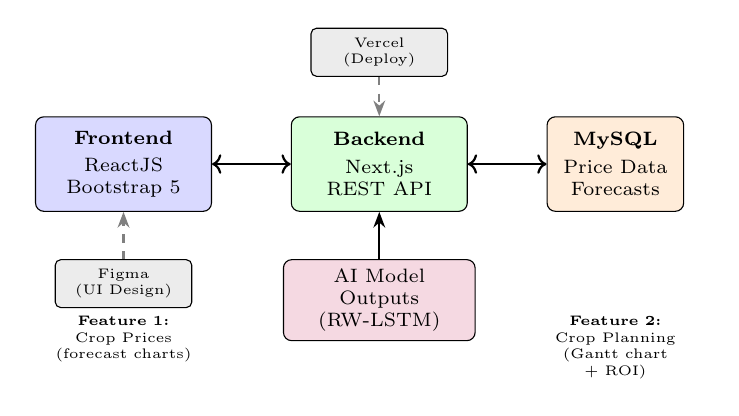
\begin{tikzpicture}[node distance=0.5cm and 0.8cm]
    % Frontend
    \node[block=blue!15, text width=2cm, align=center, minimum height=1.2cm] (fe) {
      \textbf{Frontend}\\[2pt]
      ReactJS\\
      Bootstrap 5
    };

    % Backend
    \node[block=green!15, right=1cm of fe, text width=2cm, align=center, minimum height=1.2cm] (be) {
      \textbf{Backend}\\[2pt]
      Next.js\\
      REST API
    };

    % Database
    \node[block=orange!15, right=1cm of be, text width=1.5cm, align=center, minimum height=1.2cm] (db) {
      \textbf{MySQL}\\[2pt]
      Price Data\\
      Forecasts
    };

    % AI Models
    \node[block=purple!15, below=0.6cm of be, text width=2.2cm, align=center] (ai) {AI Model Outputs\\(RW-LSTM)};

    % Figma
    \node[smallblock=gray!15, below=0.6cm of fe, text width=1.5cm, align=center] (figma) {Figma\\(UI Design)};

    % Deploy
    \node[smallblock=gray!15, above=0.5cm of be, text width=1.5cm, align=center] (vercel) {Vercel\\(Deploy)};

    % Arrows
    \draw[arrow, <->] (fe) -- (be);
    \draw[arrow, <->] (be) -- (db);
    \draw[arrow] (ai) -- (be);
    \draw[arrow, dashed, gray] (figma) -- (fe);
    \draw[arrow, dashed, gray] (vercel) -- (be);

    % Features
    \node[below=1.2cm of fe, font=\tiny, text width=2.2cm, align=center] (f1) {\textbf{Feature 1:} Crop Prices\\(forecast charts)};
    \node[below=1.2cm of db, font=\tiny, text width=2.2cm, align=center] (f2) {\textbf{Feature 2:} Crop Planning\\(Gantt chart + ROI)};
  \end{tikzpicture}}%
  \caption{Web application architecture. The frontend communicates with a Next.js backend connected to MySQL for data storage. AI model outputs feed into the backend for real-time recommendations.}
  \label{fig:webapp}
\end{figure}

The CropPlanner web application was built with ReactJS and Bootstrap~5 for the frontend, Next.js with MySQL for the backend, prototyped in Figma, and deployed on Vercel. It provides two main features: (1)~\textbf{Crop Prices}---displaying AI-predicted price charts for all four crops; and (2)~\textbf{Crop Planning}---accepting start month and area inputs, then presenting a Gantt chart recommendation with financial summaries (income, expenses, profit, and ROI).

% ============================================================
% V. RESULTS
% ============================================================
\section{Results}

\subsection{Model Comparison}

Tables~\ref{tab:mape} and~\ref{tab:accuracy} present MAPE and Accuracy results for the 2024 test year. Bold values indicate the best result per crop.

\begin{table}[htbp]
  \centering
  \caption{MAPE (\%) for 2024 Test Year}
  \label{tab:mape}
  \begin{tabular}{lcccc}
    \toprule
    \textbf{Crop} & \textbf{LSTM} & \textbf{Trans.} & \textbf{ARIMA} & \textbf{RW-LSTM} \\
    \midrule
    Cassava    & \textbf{4.81}  & 9.32  & 24.71 & 5.43  \\
    Corn       & \textbf{6.43}  & 15.09 & 8.10  & 12.06 \\
    Green Bean & 7.20           & 6.34  & 6.08  & \textbf{5.23} \\
    Soybean    & 9.44           & \textbf{5.71} & 6.99 & 6.15 \\
    \midrule
    \textbf{Average} & \textbf{7.07} & 9.12 & 11.47 & 7.22 \\
    \bottomrule
  \end{tabular}
\end{table}

\begin{table}[htbp]
  \centering
  \caption{Accuracy (\%) for 2024 Test Year}
  \label{tab:accuracy}
  \begin{tabular}{lcccc}
    \toprule
    \textbf{Crop} & \textbf{LSTM} & \textbf{Trans.} & \textbf{ARIMA} & \textbf{RW-LSTM} \\
    \midrule
    Cassava    & \textbf{95.33} & 89.99 & 77.74 & 94.57 \\
    Corn       & \textbf{93.29} & 84.29 & 92.03 & 87.95 \\
    Green Bean & 92.51          & 93.50 & 93.45 & \textbf{94.77} \\
    Soybean    & 90.57          & \textbf{94.18} & 92.82 & 93.85 \\
    \midrule
    \textbf{Average} & \textbf{92.93} & 90.49 & 89.01 & 92.79 \\
    \bottomrule
  \end{tabular}
\end{table}

No single model dominates across all crops. Standard LSTM achieves the highest average accuracy (92.93\%) and performs best for cassava and corn. Rolling-Window LSTM leads for green bean (94.77\%), while Transformer excels for soybean (94.18\%). ARIMA performs notably poorly for cassava (77.74\%) due to structural breaks violating stationarity assumptions.

\figplaceholder{Fig.~10: RW-LSTM Prediction --- Cassava (Best Case)}{Actual vs.\ predicted prices. Peak: Actual = 3.65 (Jan), Forecast = 3.51 (Feb). \textit{(Replace with actual plot)}}

\figplaceholder{Fig.~11: RW-LSTM Prediction --- Corn (Challenging Case)}{Peak predicted 3~months early. \textit{(Replace with actual plot)}}

\subsubsection{Peak Timing Accuracy}

While Rolling-Window LSTM has a slightly higher average MAPE than Standard LSTM, its key advantage is peak timing accuracy (Table~\ref{tab:peak}).

\begin{table}[htbp]
  \centering
  \caption{Peak Timing Accuracy --- Rolling-Window LSTM}
  \label{tab:peak}
  \begin{tabular}{lccccc}
    \toprule
    \textbf{Crop} & \textbf{Actual} & \textbf{Pred.} & $\boldsymbol{\Delta}$\textbf{Mo.} & $\boldsymbol{\Delta}$\textbf{Price} & \textbf{Rating} \\
    \midrule
    Cassava    & Jan & Feb & 1 & 3.93\% & Excellent \\
    Corn       & Jul & Apr & 3 & 7.52\% & Good \\
    Green Bean & Sep & Aug & 1 & 5.56\% & Excellent \\
    Soybean    & Apr & Mar & 1 & 3.46\% & Excellent \\
    \bottomrule
  \end{tabular}
\end{table}

Three of four crops have peak predictions within one month of actual values---critical for the scheduling system where peak position determines harvest dates.

\subsection{Crop Planning Results}

\figplaceholder{Fig.~12: Price Overlap Chart}{Normalized prices on common scale (log) showing peaks in different months. \textit{(Replace with actual plot)}}

The price overlap analysis reveals that peak prices for the four crops occur in different months, enabling crop rotation. The unoptimized Gantt chart (Fig.~13), where each crop is placed at its peak-optimal position, shows that green bean and corn overlap during August--December 2024.

\figplaceholder{Fig.~13: Unoptimized Gantt Chart (v1)}{Green Bean and Corn overlap. \textit{(Replace with optimal.png)}}

After applying the Greedy Scheduling algorithm, green bean was shifted from Sep--Dec to May--Aug using Strategy~B, resolving the overlap (Fig.~14).

\figplaceholder{Fig.~14: Optimized Gantt Chart (v2)}{No overlap; Green Bean shifted (dashed border). \textit{(Replace with optimize.png)}}

Table~\ref{tab:income_detail} details the income before and after optimization.

\begin{table}[htbp]
  \centering
  \caption{Income Comparison: Before vs.\ After Optimization}
  \label{tab:income_detail}
  \begin{tabular}{lcccc}
    \toprule
    \textbf{Crop} & \textbf{Before} & \textbf{After} & \textbf{Strategy} & $\boldsymbol{\Delta}$ \\
    \midrule
    Cassava    & 12,180 & 12,180 & Original & $\pm$0 \\
    Soybean    & 5,895  & 5,895  & Original & $\pm$0 \\
    Green Bean & 6,252  & 6,187  & Shifted  & $-$65  \\
    Corn       & 17,115 & 17,115 & Original & $\pm$0 \\
    \midrule
    \textbf{Total} & \textit{Infeasible} & \textbf{41,377} & --- & --- \\
    \bottomrule
  \end{tabular}
\end{table}

Green bean lost only 65~THB ($-$1.04\%) from the shift, while the total feasible income reached 41,377~THB/rai/year. Table~\ref{tab:mono} compares this with monoculture baselines.

\begin{table}[htbp]
  \centering
  \caption{Optimized Multi-Crop Rotation vs.\ Monoculture}
  \label{tab:mono}
  \begin{tabular}{lcc}
    \toprule
    \textbf{Plan} & \textbf{THB/rai/yr} & \textbf{vs.\ Opt.} \\
    \midrule
    \textbf{4-Crop Rotation} & \textbf{41,377} & --- \\
    Mono: Corn (best) & 17,115 & $+$141.7\% \\
    Mono: Cassava & 12,180 & $+$239.7\% \\
    Mono: Green Bean & 6,252  & $+$561.7\% \\
    Mono: Soybean & 5,895  & $+$601.6\% \\
    \bottomrule
  \end{tabular}
\end{table}

The optimized four-crop rotation yields approximately 2.4~times the income of the best single-crop monoculture option (corn).

\subsection{Web Application}

\figplaceholder{Fig.~15: CropPlanner --- Crop Prices Page}{Predicted price charts for all four crops. \textit{(Replace with screenshot)}}

\figplaceholder{Fig.~16: CropPlanner --- Crop Planning Page}{Input $\rightarrow$ Gantt Chart $\rightarrow$ Financial Results. \textit{(Replace with screenshot)}}

The CropPlanner web application is responsive across desktop and mobile devices. Farmers select a start month and plot area; the system displays a Gantt chart with a financial summary including income, expenses, profit, and ROI.

% ============================================================
% VI. DISCUSSION
% ============================================================
\section{Discussion}

\subsection{No Single Model Dominates}

The finding that no single model is best for all crops is attributable to the limited dataset ($\sim$252 data points) and differing price dynamics. LSTM, with fewer parameters, avoids overfitting and performs best for cassava and corn. Transformer's self-attention captures complex seasonal patterns for soybean. ARIMA fails for cassava (MAPE = 24.71\%) due to structural breaks violating stationarity, but remains competitive for crops with regular trends.

\subsection{Peak Timing Over Overall MAPE}

Rolling-Window LSTM's average MAPE (7.22\%) is slightly higher than Standard LSTM (7.07\%) because it must generalize across multiple windows. However, its superior peak timing accuracy (3/4~crops $\leq$1~month off) makes it the preferred choice for scheduling, where an incorrect peak shifts the entire Gantt chart. In production, an ensemble approach selecting the best model per crop would be ideal.

\subsection{Greedy Scheduling Sufficiency}

The greedy heuristic does not guarantee global optimality---scheduling a high-income crop first may block two medium-income crops with higher combined revenue. With only four crops ($4! = 24$ permutations), greedy performs well; green bean lost merely 65~THB ($-$1.04\%). For $>$10~crops, Dynamic Programming in $O(n \log n)$ would be necessary.

\subsection{Experimental Design Limitations}

A single test year (2024) may not capture model stability. The absence of a validation set, while justified by fixed hyperparameters, risks undetected overfitting. Multi-year rolling evaluation would provide more robust conclusions.

% ============================================================
% VII. LIMITATIONS AND FUTURE WORK
% ============================================================
\section{Limitations and Future Work}

This study has several limitations: (1)~a single test year with no validation set; (2)~no field testing with actual farmers; (3)~external factors (weather, policy, global prices) are not modeled; (4)~greedy scheduling does not guarantee optimality; (5)~coverage is limited to Northeastern Thailand and four crops.

Future directions include: (1)~ensemble model selection per crop; (2)~multi-year rolling evaluation; (3)~incorporating weather and economic features; (4)~Dynamic Programming for $>$10 crops; (5)~user studies with farmers; (6)~expanding regional and crop coverage.

% ============================================================
% VIII. CONCLUSION
% ============================================================
\section{Conclusion}

This paper presented CropPlanner, an integrated system for AI-driven crop planning. Three contributions were made:

First, a comparative study of four forecasting models revealed that no single model dominates across all metrics. Standard LSTM achieved the highest average accuracy (92.93\%), while Rolling-Window LSTM exhibited superior peak timing accuracy---predicting peaks within one month for three of four crops.

Second, the Greedy Scheduling algorithm produced a non-overlapping four-crop rotation yielding 41,377~THB/rai/year---approximately 2.4~times the best monoculture income.

Third, the CropPlanner web application enables farmers to plan up to 12~months ahead through intuitive visualizations.

This system has the potential to reduce income volatility, distribute earnings throughout the year, and promote sustainable agriculture for Thai farmers.

% ============================================================
% REFERENCES
% ============================================================
\begin{thebibliography}{14}

\bibitem{oae2024stats}
Office of Agricultural Economics (OAE), ``Agricultural Statistics of Thailand,'' Ministry of Agriculture and Cooperatives, Bangkok, 2024.

\bibitem{oae2024forecast}
OAE, ``Crop Production Forecast Report,'' Ministry of Agriculture and Cooperatives, Bangkok, 2023/2024.

\bibitem{ocsb2024}
Office of the Cane and Sugar Board, ``Annual Report of Sugarcane and Sugar Industry,'' Ministry of Industry, Bangkok, 2024.

\bibitem{thairice2024}
Thai Rice Export Association, ``Thai Rice Export Statistics,'' Ministry of Agriculture and Cooperatives, Bangkok, 2024.

\bibitem{waqas2024climate}
M.~Waqas \textit{et al.}, ``A comprehensive review of the impacts of climate change on agriculture in Thailand,'' \textit{Res.\ Environ.\ Sustain.}, vol.~16, 100152, 2024.

\bibitem{asg2014}
Academic Service Group~2, ``Report on Agricultural Price Depression Problems,'' Secretariat of the House of Representatives, Bangkok, 2014.

\bibitem{rohan2025crop}
R.~Rohan \textit{et al.}, ``Improving Crop Price Prediction Using Machine Learning,'' \textit{ResearchGate}, 2025.

\bibitem{javaid2023ai}
M.~Javaid \textit{et al.}, ``Understanding the potential applications of Artificial Intelligence in agriculture sector,'' \textit{Adv.\ Agrochem.}, vol.~2, no.~1, pp.~15--30, 2023.

\bibitem{kkm2023rice}
K.~K.~M, ``Exponential Smoothing Model and Evaluation of Rice,'' \textit{IJISRT}, vol.~8, no.~5, 2023.

\bibitem{hochreiter1997lstm}
S.~Hochreiter and J.~Schmidhuber, ``Long Short-Term Memory,'' \textit{Neural Comput.}, vol.~9, no.~8, pp.~1735--1780, 1997.

\bibitem{vaswani2017attention}
A.~Vaswani \textit{et al.}, ``Attention is All You Need,'' in \textit{Proc.\ NeurIPS}, 2017, pp.~5998--6008.

\bibitem{boxjenkins}
G.~E.~P.~Box and G.~M.~Jenkins, \textit{Time Series Analysis: Forecasting and Control}. San Francisco: Holden-Day, 1976.

\bibitem{pinch2020scheduling}
[REF --- Job scheduling / optimization in agriculture]

\bibitem{rossi2021dss}
[REF --- Decision support systems in agriculture]

\end{thebibliography}

\end{document}